% compile with: pdflatex -shell-escape filename.tex
\documentclass[crop,tikz,convert=pdf2svg]{standalone}
\usetikzlibrary{shapes.geometric}

\tikzstyle{node}=[
	circle,
	draw=black,
	minimum size=0.75cm,
	thick,
]

\tikzstyle{subtree}=[
	draw=black,
	minimum size=1.75cm,
  regular polygon sides=3,
  regular polygon,
]

\begin{document}

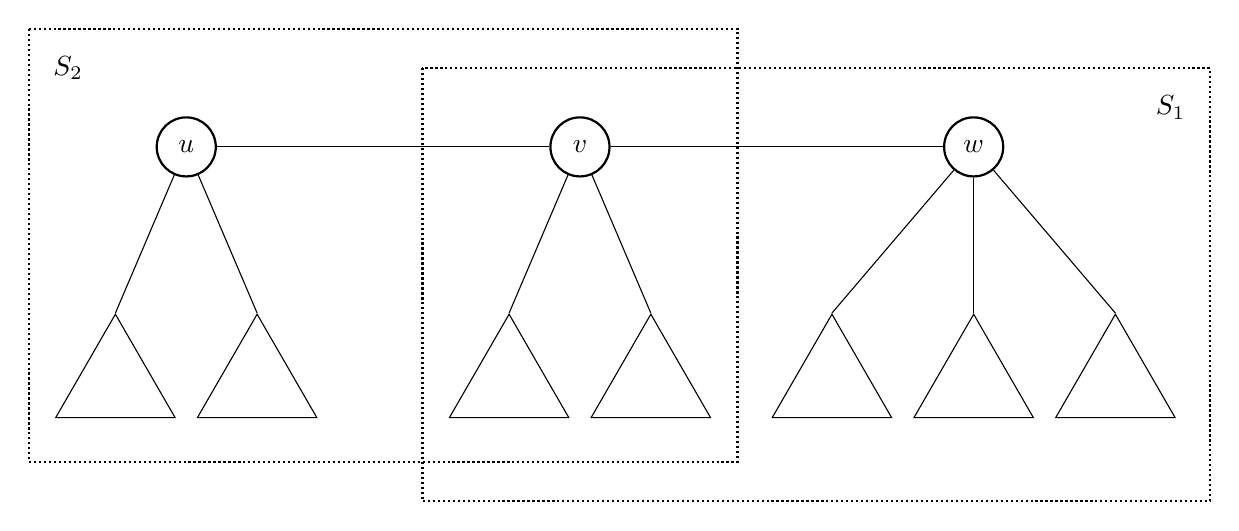
\begin{tikzpicture}
  \node[node] (u) at (0,0) {$u$};
  \node[node] (v) at (5,0) {$v$};
  \node[node] (w) at (10,0) {$w$};

  \node[subtree] (s1) at (-0.9,-3) {};
  \node[subtree] (s2) at (0.9,-3) {};
  \node[subtree] (s3) at (4.1,-3) {};
  \node[subtree] (s4) at (5.9,-3) {};
  \node[subtree] (s5) at (8.2,-3) {};
  \node[subtree] (s6) at (10,-3) {};
  \node[subtree] (s7) at (11.8,-3) {};

  \draw (u) -- (v) -- (w);
  \draw (s1.north) -- (u);
  \draw (s2.north) -- (u);
  \draw (s3.north) -- (v);
  \draw (s4.north) -- (v);
  \draw (s5.north) -- (w);
  \draw (s6.north) -- (w);
  \draw (s7.north) -- (w);

  \draw[densely dotted,thick] (-2,1.5) rectangle (7,-4);
  \node at (-1.5, 1) {$S_2$};
  \draw[densely dotted,thick] (3,1) rectangle (13,-4.5);
  \node at (12.5, 0.5) {$S_1$};
\end{tikzpicture}

\end{document}
